\documentclass[a4paper, 12pt]{article}
\usepackage[left=2.5cm,right=2.5cm,top=2.5cm,bottom=2.5cm,includeheadfoot]{geometry}
\usepackage{graphicx}
%\usepackage[T1]{fontenc}
\usepackage{amssymb}
%\renewcommand{\familydefault}{\sfdefault}
\usepackage{lmodern}
\usepackage{amsmath}
\usepackage{wrapfig}
\usepackage{etoolbox}
\usepackage{nth}
\usepackage{url}

% tipa for IPA symbols, added by TS, 27-10-2014
\usepackage{tipa}


\usepackage{setspace}
\onehalfspacing

\usepackage{picins}
\usepackage[font=scriptsize,labelfont=bf]{caption}
\usepackage{hyperref}

\usepackage[utf8]{inputenc}

\usepackage[round,authoryear]{natbib}


\hypersetup{
  colorlinks   = true, %Colours links instead of ugly boxes
  urlcolor     = blue, %Colour for external hyperlinks
  linkcolor    = blue, %Colour of internal links
  citecolor   = blue %Colour of citations
}
   

\title{Working with EMA data files in MATLAB}
\date{\today}
\author{Jens Roeser, Tanner Sorensen \& Adamantios Gafos$^{*}$\vspace{0.5mm}\\
Department of Linguistics, University of Potsdam\\
$^{*}$email: \href{mailto:jens.roes@gmail.com}{
gafos@uni-potsdam.de}}

\begin{document}

\maketitle
\thispagestyle{empty}
\newpage


\section{Introduction}\label{sec:struc}

This guide describes how to handle data structures containing data from electromagnetic articulography (EMA) in MATLAB. We are presupposing basic MATLAB working experience. However, all necessary information to work with EMA data in MATLAB are included. We will make reference to programming concepts like data types, which we consider important for working with data. However, since we do not elaborate on data type concepts (we merely tell the reader what these types are and carry on with our narrow interests in this guide), we remind the reader of the \href{http://www.mathworks.de/de/help/matlab/structures.html}{MathWorks} homepage for further information. There is of course a wealth of introductions to MATLAB, such as  \cite{attaway2012}, \cite{gilant2011}, and \cite{rosenbaum2012}, if the reader feels unable to follow the MATLAB coding herein. \cite{quarteroni2010} is recommended for readers with interests beyond the scope of the present guide.

In this guide, we  focus on data sets that are provided by experiments carried out with the EMA method. While reading this guide, apply the provided commands in your MATLAB console or from a script to an available binary \texttt{.mat} EMA data file. Type the commands rather than copy-paste them. Solve the included tasks to understand the structure of EMA data files and how to extract relevant information.

EMA data files have a \texttt{.mat} extension and contain acoustic and articulatory information. These files are data structures which are called structure arrays -- a particular data type in MATLAB. A structure array is a collection of information of different types (e.g., strings, also known as character arrays, or numbers like integers or floating-point numeric data) and different lengths all yoked together in one object (here, usually a stimulus elicited from a participant in our experiments). Inside such data structures there are fields each containing a subset of the data (the movement in time of one sensor or another or the acoustic waveform). We will make this more concrete in what follows. In contrast to cell arrays, a structure array has one name for many data subsets (here, different trajectories and the audio waveform). 

\newpage
\section{Data structure}\label{sec:emastruc}

If the relevant EMA data file that you are going to work with is contained in your current working directory, the \texttt{load} function can be used to get the file into the MATLAB working environment. The name of the data file with \texttt{.mat} extension must be given to the function as argument. Note that the name must be a string in single quotes. If the file is located somewhere else, the entire path or a relative path (relative to the current directory) to that file must be given as an argument. The structure array is assigned to the variable \texttt{file} using the equal sign. \texttt{file} now contains a 1$\times$1 structure array with only one element. We will see in a bit that an 1$\times$7 structure array is embedded in this element and can be accessed for processing.\footnote{Unfortunately, the single quotes used in the commands throughout this guide are not the same characters as those corresponding to what MATLAB considers to be a quote, due to the \LaTeX{} compilation. Thus, if you were to copy and paste the commands used in this report into the MATLAB console, you will see \texttt{Error: The input character is not valid in MATLAB statements or expressions}. Change the quotes in the copied command by entering single quotes from your keyboard.} The double arrows \texttt{>>} indicate a command to be given to MATLAB by you, the user. The lines without these arrows indicated a MATLAB-generated echo. Do not copy \texttt{>>} when copying the code in the MATLAB command window.

\begin{verbatim}
>> file = load(`cascade_09_0823.mat')

file = 

    cascade_09_0823: [1x7 struct]
\end{verbatim}

If you think it is annoying to type long file names to load data, the names of the files in your directory can be accessed using \texttt{dir} as in the code below. This command returns the names of and information about the files in a directory. The asterisks $\ast$ is used as a wild card assigning only the files that end in \texttt{.mat} as specified in the string below to the variable \texttt{list}. The \texttt{.mat} files in your current working directory will be listed in an n$\times$1 structure array with n being the number of files in the current directory and the first field of the returned structure array being the file name. The other fields are not relevant here. Fields in a structure array can be accessed using a dot \texttt{.} after the name of the structure array and before the field name that must be accessed shown in the line after. Curly brackets \texttt{\{\}} return all information listed in the \texttt{name} field being the names of the \texttt{.mat} files in your current working directory.

\begin{verbatim}
>> list = dir(`*.mat')

list = 

4x1 struct array with fields:
    name
    date
    bytes
    isdir
    datenum

>> {list.name}

ans = 

  Columns 1 through 2

    'cascade_09_0823.mat'    'cascade_10_0865.mat'

  Columns 3 through 4

    'clean_01_0048.mat'    'clean_02_0152.mat'
\end{verbatim}

Like we did above, the first file listed in \texttt{list.name} can be loaded with the \texttt{load} function. To load this file, the structure array \texttt{list}'s field name is indexed by 1 for the first file like shown below. Again, the data are encapsulated in a 1$\times$1 structure array with one field named after the file (without extension). 

\begin{verbatim}
>> file = load(list(1).name)

file = 

    cascade_09_0823: [1x7 struct]
\end{verbatim}

This was an alternative way to load a file into MATLAB. Now we are back from where we started before -- an EMA file has been loaded. This alternative way to load data is more flexible for loading multiple files and avoids annoying typing of long file names.\par %Feel free to try this by simply writing a loop around the following command and replacing 1 by an iteration index (e.g., i)


\texttt{file} is a variable which we set equal to whatever MATLAB data structure corresponds to the file \texttt{cascade\_09\_0823.mat}. Each variable in MATLAB (and any programming environment) is of a specific Class (or Type). The type of this variable is what MATLAB refers to as a \texttt{struct array}. You can see the type above in the \texttt{[1x7 struct]} part or you can ask MATLAB to give you the type using the \texttt{whos} command below. Note, that it is often important to keep track of the data type.

\begin{verbatim}
>> whos file
  Name      Size             Bytes  Class     Attributes

  file      1x1             591104  struct              
\end{verbatim}

We do not know what and how information is stored in \texttt{file}. To find that out, we need to know the \textit{fields} of the structure (because in MATLAB structure arrays are data structures that store information in separate fields). To get to know what these fields are, we apply the function \texttt{fieldnames} to \texttt{file} which returns a cell array of strings containing the structure field names associated with some structure. The \texttt{help} function gives the basic information about the function of interest.

\begin{verbatim}
>> help fieldnames

 FIELDNAMES Get structure field names.
    NAMES = FIELDNAMES(S) returns a cell array of strings containing 
    the structure field names associated with the structure s.

>> names = fieldnames(file)

names = 

    'cascade_09_0823'
\end{verbatim}

It just happens that our structure array assigned to \texttt{file} actually has just one field and the name of the field is the name of the file itself. That is not always the case. It could be that the structure array has more than one field (e.g., \texttt{date}, `date data were collected', \texttt{rate}, `sampling rate' and so on for \texttt{list} above. Since now we know the field name of our structure array, we can ask to see its content by using the function \texttt{getfield} below with the structure array \texttt{file} as its first argument, and the name of the file as its second argument.

\begin{verbatim}
>> help getfield

 GETFIELD Get structure field contents.
    F = GETFIELD(S,'field') returns the contents of the specified
    field.

>> data = getfield(file, names{1})

data = 

1x7 struct array with fields:
    SIGNAL
    SRATE
    NAME
\end{verbatim}

We have learned above that the function \texttt{fieldnames} gives us a cell array of strings, and for cell arrays one needs to use curly brackets \texttt{\{\}} to access any specific entry in the cell array and since we want to access the first entry here we need to write \texttt{names\{1\}} to retrieve the first file.\par
\texttt{data} contains a 1$\times$7 structure array with the fields \texttt{SIGNAL}, \texttt{SRATE}, and \texttt{NAME}. This may differ from your output, since EMA data files contain different kind and amount of information. Each of the seven entries of the structure array contains one field for the audio signal and six fields for movement trajectories. To see which signals are available, the field \texttt{NAME} can be accessed like in above for the files in \texttt{list}. Here, the field \texttt{NAME} is accessed in the structure array \texttt{data}. The values of the field \texttt{NAME} are returned as strings and assigned to the variable \texttt{trajectories} (which is a cell array of strings).\par

\begin{verbatim}
>> trajectories = {data.NAME} 

ans = 

  Columns 1 through 6

    'audio'    'TBPOS'    'TMPOS'    'TTPOS'    'LLPOS'    'ULPOS'

  Column 7

    'JAWPOS'
\end{verbatim}

\noindent \textbf{Exercise 1:} The field \texttt{SRATE} contains information about the sampling rate used during the data recording. As we have done with the file names and signal names before, check which sampling rate has been used for audio and for the individual trajectories by changing the previous command (i.e., instead of asking for the \texttt{NAME} field, ask for the \texttt{SRATE} field).\footnote{Note that field names are in capital letters.}\par\smallskip

\newpage
\section{Signal processing}
\subsection{Spatial signals}\label{spasig}

The field \texttt{SIGNAL} contains the signal that is discretized as sequence of values called samples, each spanning a small time slice as determined by the sampling rate. \texttt{SIGNAL} contains positional values for the x-\,and y-dimension of the tongue kinematics for 2D data files and additionally the z-dimension for 3D data files. Structure array information of single signals can be accessed using the column number from above, which is the corresponding field name. The names of each signal have been assigned to the variable \texttt{trajectories}. The following code shows how to find the index of the desired signal using \texttt{strmatch}. This function takes the name of the signal (here, \texttt{TBPOS} which is the tongue back posture) as first argument and the vector with the signal names \texttt{trajectories} as second argument. This will provide an index saved in \texttt{idx} (here, \texttt{2}) that can be used as an index for \texttt{data} corresponding to the signal name \texttt{TBPOS}. 

\begin{verbatim}
>> idx = strmatch('TBPOS', trajectories, 'exact')

idx =

     2

>> data(idx)

ans = 

    SIGNAL: [928x2 double]
     SRATE: 400
      NAME: 'TBPOS'
\end{verbatim} 

\texttt{NAME} shows the trajectory's name, \texttt{SRATE} is the sampling frequency (here, 400 Hz) used to record \texttt{TBPOS}. \texttt{SIGNAL} is a 928$\times$2 matrix with 928 rows and 2 columns. The column number represents the x and y positional signals of the sensor glued on the tongue body and the row number corresponds to one row for each recorded sample (i.e., 928 samples for this file). The command below returns the signal of the x-\,and y-dimension for the first 5 values of \texttt{TBPOS} using indexing \texttt{1:5}, i.e.\,row 1 to 5 and all (i.e., both) columns using colon \texttt{:}. Indexing in MATLAB and many other environments takes first the row index and then the column index. The left column shows the x-values and the right column the y-values. Again, every row or pair of values below corresponds to one sample of the position of the sensor in 2D. The \texttt{SIGNAL} values of \texttt{TBPOS} are saved in a vector matrix \texttt{signal\_tbp}.

\begin{verbatim}
>> data(2).SIGNAL(1:5,:)

ans =

   42.4871   -5.1379
   42.4776   -5.1641
   42.4686   -5.1885
   42.4603   -5.2097
   42.4531   -5.2264

>> signal_tbp = data(2).SIGNAL;
\end{verbatim}

\noindent \textbf{Exercise 2:} Repeat the same for the tongue tip trajectory (i.e., \texttt{TTPOS}). Use \texttt{strmatch} for \texttt{TTPOS} instead of \texttt{TBPOS} and index \texttt{data}. Then, find the positional values x and y of the 266$^{\text{th}}$ sample in the \texttt{TTPOS} trajectory. You can access positional values using \texttt{data(n).SIGNAL(r,c)} by replacing \texttt{n} with the field number of the trajectory name, \texttt{r} with the row number which is the sample index, and \texttt{c} with the column (i.e., 1 for x-values, 2 for y-values and for 3D data, 3 for z-values).\par\smallskip

Speech signals (audio or kinematics) are stored as sequences of samples. These samples are taken at regular time intervals, whose regularity is expressed by a certain sampling rate or frequency. Frequency is the number of cycles of a periodic process (here, the sampling process) in one second, i.e. how many times the process repeats itself in one second. Frequency is expressed in units of Hz, with 1 Hz corresponding to one cycle per second. One property of a speech signal is its duration which is often expressed in real-time units such as seconds or milliseconds (msec). To convert from samples to duration, we need to know the frequency at which our signal was sampled. Equation \eqref{eq:sf} is the well-known expression for the relation between frequency $f$ (in Hz) and period $T$ (in seconds) of a repeating process. Hence, to find the duration $t$ of a sampled signal in seconds we divide the number of samples $n$ by the sampling rate $f$ as in equation \eqref{eq:t}. Conversely, if we know the duration or time stamp $t$ in our signal and we would like to compute the number of samples $n$ corresponding to that duration or time stamp, we do so by taking the product of duration $t$ and the sampling frequency $f$ as shown in equation \eqref{eq:s}. We will give MATLAB code for equations \eqref{eq:t} and \eqref{eq:s} below, when we need to compute the time stamp corresponding to some sample number or the sample number corresponding to some time stamp.

\begin{equation}
f = 1/T  \label{eq:sf}
\end{equation}
\begin{equation}
t = n/f  \tag{\ref*{eq:sf}$^\prime$}\label{eq:t}
\end{equation}
\begin{equation}
n = t^{*}f  \tag{\ref*{eq:sf}$^{\prime\prime}$}\label{eq:s}
\end{equation}

Let us apply these notions to finding the duration in msecs of one of our signals \texttt{TBPOS} with the following code. The total number of rows (samples) stored in the field \texttt{SIGNAL} can be found using the \texttt{length} function. We subtract 1 from that and divide the term by the signal's sampling rate \texttt{SRATE} (see equation \eqref{eq:t}). Finally, we multiply this expression by 1000 to convert from seconds to msecs. The reason for the subtraction by 1 is conventional: The first sample should correspond to 0 msecs. More explicitly, the sampling rate for \texttt{TBPOS} is 400 Hz (try \texttt{data(2).SRATE}). This means that a sample is taken every 0.0025 seconds (try \texttt{1/data(2).SRATE}) or every 2.5 msecs.  If \texttt{length} returns 1 as the number of samples in our data file, the formula below would give 0 msec; for 2 samples, the formula would return 2.5 msec; for 3, 5 msec; for 4, 7.5 msec and so on.\footnote{Note: In the formula output, MATLAB gives us \texttt{2.3175e+03} in scientific notation, that is, 2.3175 multiplied by a power-of-10 scale factor, here multiply by 1000, i.e., 2317.5 msec.}


\begin{verbatim}
>> dur = 1000*(length(data(2).SIGNAL)-1)/data(2).SRATE

dur =

   2.3175e+03
\end{verbatim}

\setlength\intextsep{-10pt}
\begin{wrapfigure}[9]{R}{6.3cm}
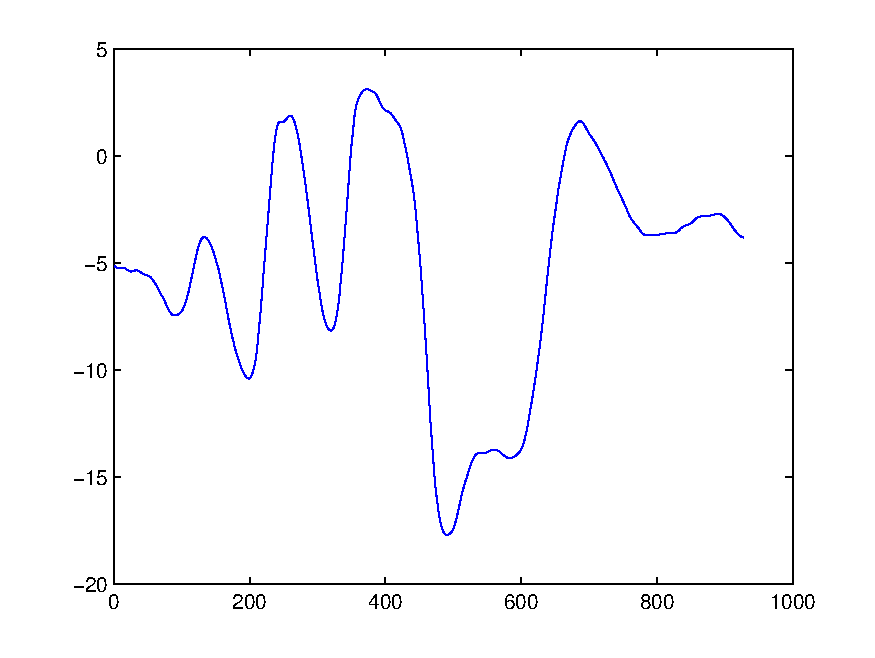
\includegraphics[scale=0.45]{TBPOS.pdf}%width=6cm, height=4cm
\caption{Signal of \texttt{TBPOS} in y-diminsion.}\label{fig:tbpos}
\end{wrapfigure}
               
We now visualize individual sensor positional signals. The \texttt{TBPOS} signal can be plotted by entering the command below. \texttt{(:,2)} selects all rows of the second column which is the position of the signal in y-dimension. Again, \texttt{data(2)} refers to \texttt{TBPOS}. Figure \ref{fig:tbpos} shows the y-signal of \texttt{TBPOS} plotted against sample number. The plot shows the excursion of the tongue back sensor in the y-dimension over the course of time, which is here represented in terms of samples. % The vector matrix \texttt{signal\_tbp} defined before has not been used here, since the actual structure array provides a more flexible way to check other trajectories, dimension, and particular sample slices. 

\begin{verbatim}
>> plot(data(2).SIGNAL(:,2))
\end{verbatim}

\noindent \textbf{Exercise 3:} Create the plot in Figure \ref{fig:tbpos} using the vector matrix \texttt{signal\_tbp} from above. Also, plot the signal for the x-dimension of \texttt{TTPOS} by changing the relevant indices in the plot command for Figure \ref{fig:tbpos}. Remember, \texttt{data.NAME} gives the trajectory names for the index of \texttt{TTPOS}.\par\smallskip

\setlength\intextsep{-5pt}
\begin{wrapfigure}[10]{R}{6.3cm}
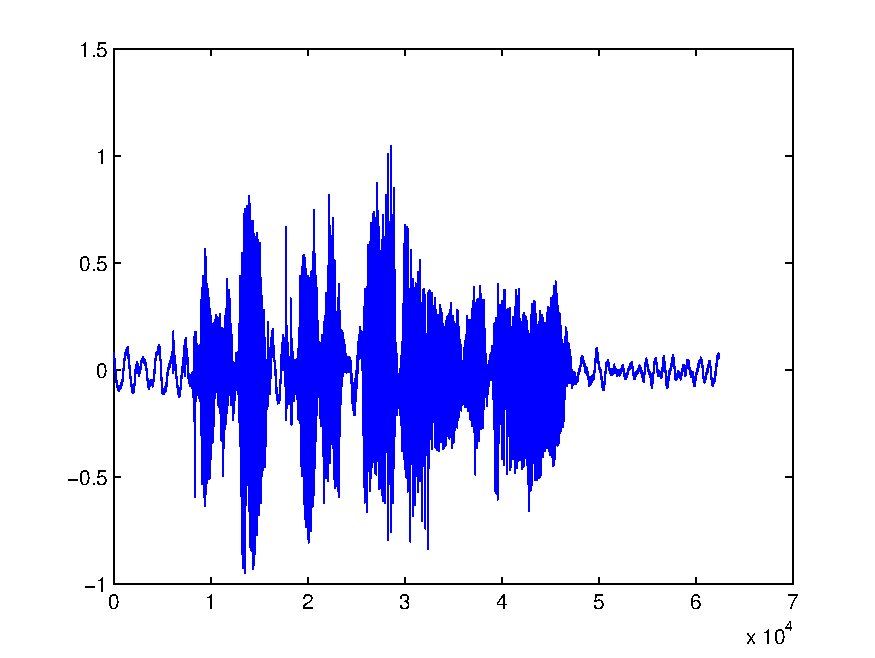
\includegraphics[scale=0.45]{wave.pdf}%width=6cm, height=4cm
\caption{Mono waveform of the audio array over samples.}\label{fig:wave}
\end{wrapfigure}

As we saw above, the audio information is contained in the first field of the structure array. Applying the \texttt{soundsc} function below to the signal information of audio as the first argument and the corresponding sampling rate as the second argument the sound of the file can be played. \texttt{soundsc} scales the values of the audio signal to the range from $-1.0$ to 1.0, and sends the data to the speaker at the given sample rate 25600 Hz (try, \texttt{data(1).SRATE}). The positional values of the mono waveform are the signal of the field audio with only one dimension which is shown in Figure \ref{fig:wave} using the \texttt{plot} command below. Note here that \texttt{SIGNAL}, \texttt{SRATE}, and \texttt{NAME} are fields contained in every sensor, thus for audio and all trajectories, but they differ in e.g.\,number of dimensions.
  
\begin{verbatim}
>> soundsc(data(1).SIGNAL, data(1).SRATE)
>> plot(data(1).SIGNAL)
\end{verbatim}

The x-axis in Figure \ref{fig:wave} displays samples. This is less intuitive, therefore the x-axis should be transformed to msec. The \texttt{linspace} command like shown below can be used taking three arguments. This function produces a linearly spaced vector with respect to every single row value of the signal involved between 0 as defined below and the length of the signal stored in \texttt{signal\_len} as the last argument. The signal length \texttt{signal\_len} divided over the sampling rate for duration shown in equation \eqref{eq:t} as second argument defines how to linearly space the values. The output is saved in \texttt{signal\_sec} which is multiplied by 1000 for msec in the plot. Defining the duration of audio signal as the first argument plots the duration on the x-axis and the spatial signal as second argument on the y-axis. The \texttt{xlabel} function adds a label \textit{Time (msec)} to the x-axis. The returned plot is shown in Figure \ref{fig:wavems}.



\setlength\intextsep{-20pt}
\begin{wrapfigure}[8]{R}{6.3cm}
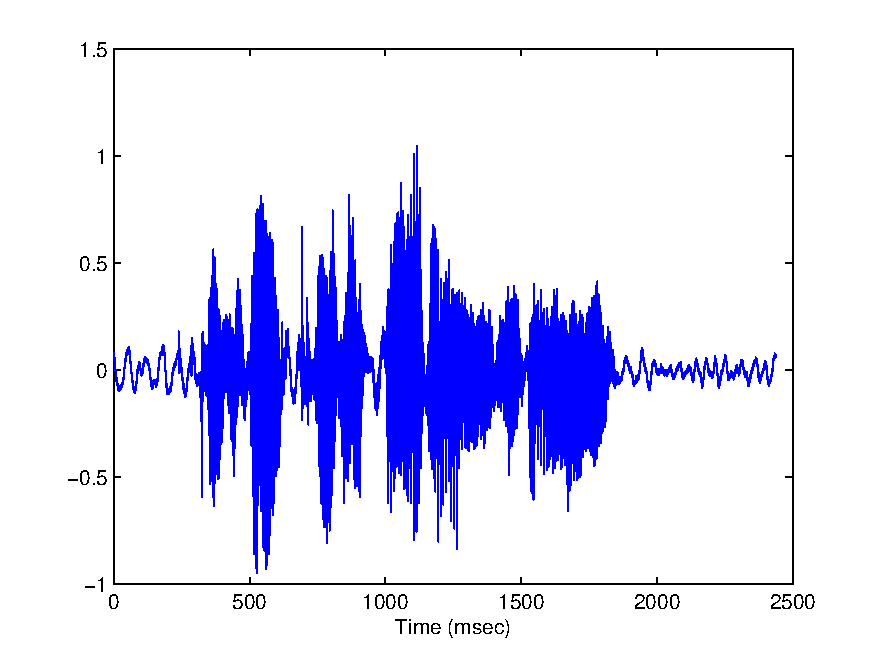
\includegraphics[scale=0.45]{wavems.pdf}%width=6cm, height=4cm
\caption{Mono waveform of the audio array plotted over time (msec).}\label{fig:wavems}
\end{wrapfigure}



\begin{verbatim}
>> signal_len = length(data(1).SIGNAL);
>> signal_sec = linspace(0, signal_len / data(1).SRATE, signal_len);
>> plot(signal_sec*1000, data(1).SIGNAL)
>> xlabel('Time (msec)')
\end{verbatim}


If the audio signal must be saved as a \texttt{.wav} file outside of the \texttt{.mat} file, the function \texttt{audiowrite} can be applied to the signal shown in the following command.\footnote{Your current MATLAB version might not yet use \texttt{audiowrite}. Use \texttt{wavwrite} instead which works equivalently.} A string must be specified as output name of the \texttt{.wav} file. Further arguments are the signal of the audio data array, and the corresponding sampling rate. In this way, the binary \texttt{.mat} structure can be converted to an audio file. 

\begin{verbatim}
>> audiowrite(`test.wav', data(1).SIGNAL, data(1).SRATE);
\end{verbatim}

\noindent\textbf{Exercise 4:} MATLAB might give you a warning here, that can be circumvented by normalizing the amplitude of the signal to 1 like shown in the code below. The normalized audio signal is assigned to \texttt{audio\_signal}. Normalize the audio signal before saving it to a \texttt{.wav} file circumventing the warning from before. You will basically have to apply the function \texttt{audiowrite} to \texttt{audio\_signal}. If you were successful, no warning should appear in the console if previously seen.\par\smallskip

\begin{verbatim}
>> audio_signal =  data(1).SIGNAL/max(abs(data(1).SIGNAL));
\end{verbatim}

The signals embedded in the structure array are synchronous. The samples (i.e., each row) have instances in all trajectories, thus, the positional values of the n$^{\text{th}}$ sample have representations in \texttt{TBPOS}, \texttt{TTPOS} and all other trajectories, and in \texttt{audio}. The trajectories contain information about the position of the tongue and lip at a particular time (i.e., sample). Therefore, given a particular sample, say 552, the positional values (x, y) for different trajectories can be extracted. For instance, the positional values for the 552 sample in the \texttt{TBPOS}, \texttt{TMPOS} (i.e., tongue mid posture), and \texttt{ULPOS} (i.e., upper lip posture) can be extracted using the respective field numbers 2, 3, and 6 to index the structure array \texttt{data}. Row 552 has been indexed for the 552$^{\text{nd}}$ sample and all columns \texttt{:} to return both the x-\,and y-value.


\begin{verbatim}
>> data(2).SIGNAL(552,:)

ans =

   39.0359  -13.8055

>> data(3).SIGNAL(552,:)

ans =

   24.5798  -10.5309

>> data(6).SIGNAL(552,:)

ans =

   -8.7424    3.4116
\end{verbatim}

\noindent\textbf{Exercise 5:} Extract the positional values (x, y) for the 432$^{\text{nd}}$ sample of JAWPOS (i.e., jaw posture), LLPOS (i.e., lower lip posture), and audio. You saw above how to get to the index of the signal fields.\par\smallskip


\subsection{Local extrema}\label{locext}

Imagine you are given a time stamp in milliseconds (e.g., 650 msec) in the vowel /a/ and you are supposed to find the time stamp corresponding to the largest deflection in y-dimension in the region around that time stamp (a local maximum). For the vowel /a/ it is reasonable to concentrate on the \texttt{TBPOS} trajectory. First, we must convert the given time stamp into the corresponding sample index shown in the code below. We start by assigning the relevant time stamp to a variable \texttt{msecs}, extract the sampling rate of \texttt{TBPOS} by accessing the field \texttt{SRATE} and assign it to \texttt{sRate}, and calculate the corresponding sample index \texttt{samps} of the given time stamp which is the product of the duration and the sampling rate as in equation \eqref{eq:s} in Section \ref{spasig}, divided by 1000 for seconds. The function \texttt{floor} truncates any decimal digits of the resulting value to the closest integer (sample numbers can only be integers) and then we add 1 analogue to the explanation in Section \ref{spasig}. The output sample index corresponds to a value on the x-axis in Figure \ref{fig:tbpos}.\footnote{Note, MATLAB is case sensitive, which means it will not confuse the field name \texttt{SRATE} of the structure array \texttt{data} and the vector \texttt{sRate}, since the first is capitalized and the latter is not.}



\begin{verbatim}
>> msecs = 650; sRate = data(2).SRATE; samps = floor(msecs*sRate/1000)+1

samps =

   261
\end{verbatim}


\setlength\intextsep{-10pt}
\begin{wrapfigure}[9]{r}{6.3cm}
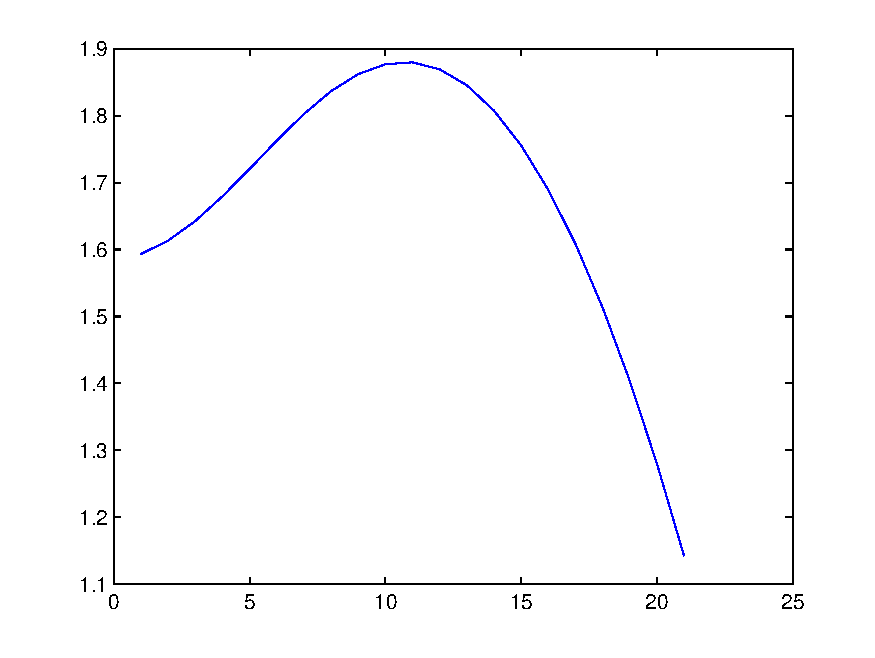
\includegraphics[scale=0.45]{localmax.pdf}%width=6cm, height=4cm
\caption{Region of \texttt{TBPOS} around 650 msec.}\label{fig:locmax}
\end{wrapfigure}




\noindent\textbf{Exercise 6:} Calculate the sample index of \texttt{TBPOS} that corresponds to a time stamp at 1200 msec. Also, calculate the sample index for \texttt{audio}. Note that we saw that the sample index of a given value in msecs depends on the sampling rate (see equation \eqref{eq:s} in Section \ref{spasig}). The sampling rate may differ for \texttt{audio} and for other signals.\par\smallskip


Let us get back to the problem from above. We are given a time stamp at 650 msec that we converted to 261 samples. In order to get an impression of the region around this value, we can plot an arbitrary region around 261 for the y-dimension in \texttt{TBPOS} as shown in the following code. The rows from 250 to 270 for the second column (y-values) have been indexed. The resulting plot in Figure \ref{fig:locmax} shows the tongue movement in y-dimension for the \texttt{TBPOS} around 650 msec.

\begin{wrapfigure}[9]{R}{6.3cm}
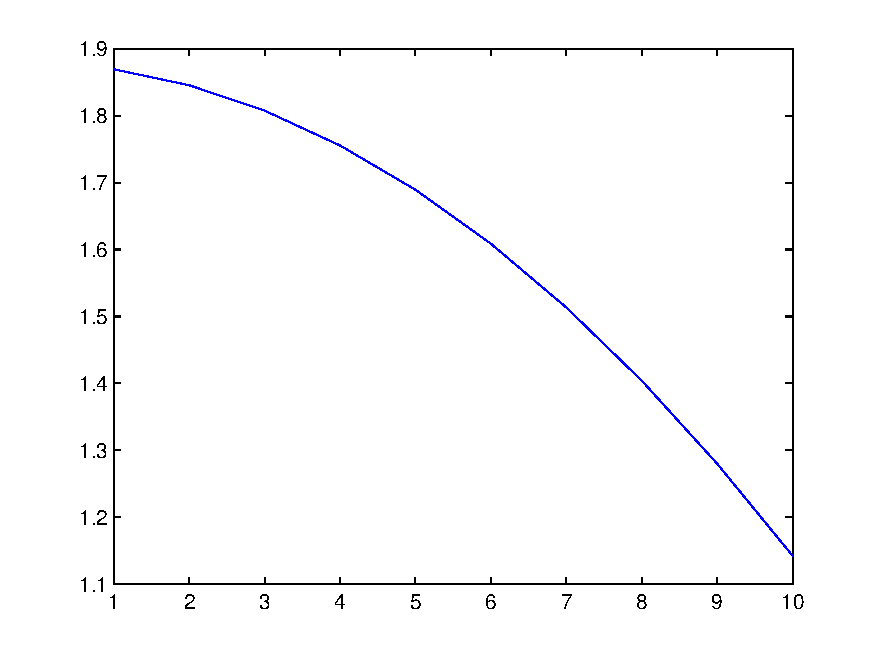
\includegraphics[scale=0.45]{increase.pdf}%width=6cm, height=4cm
\caption{Region of \texttt{TBPOS} after 650 msec.}\label{fig:increase}
\end{wrapfigure}


\begin{verbatim}
>> plot(data(2).SIGNAL(250:270,2))
\end{verbatim}

Figure \ref{fig:locmax} shows that the chosen range around the sample number corresponding to the time stamp includes a local maximum. Note that there is no guarantee that this will always be the case. For example, in Figure \ref{fig:increase} we plotted the trajectory of samples above the given time stamp with index from row 261 until 270. If a maximum is calculated for the latter region, a value at the left boundary will be returned. This may not correspond to what you would intuitively call a maximum. The range of samples chosen for Figure \ref{fig:increase} is monotonically decreasing in their y-values, and so the ``real'' maximum probably occurred at some sample before this range. 

\begin{verbatim}
>> plot(data(2).SIGNAL(261:270,2))
\end{verbatim}


\setlength\intextsep{-3pt}
\begin{wrapfigure}[10]{R}{6.3cm}
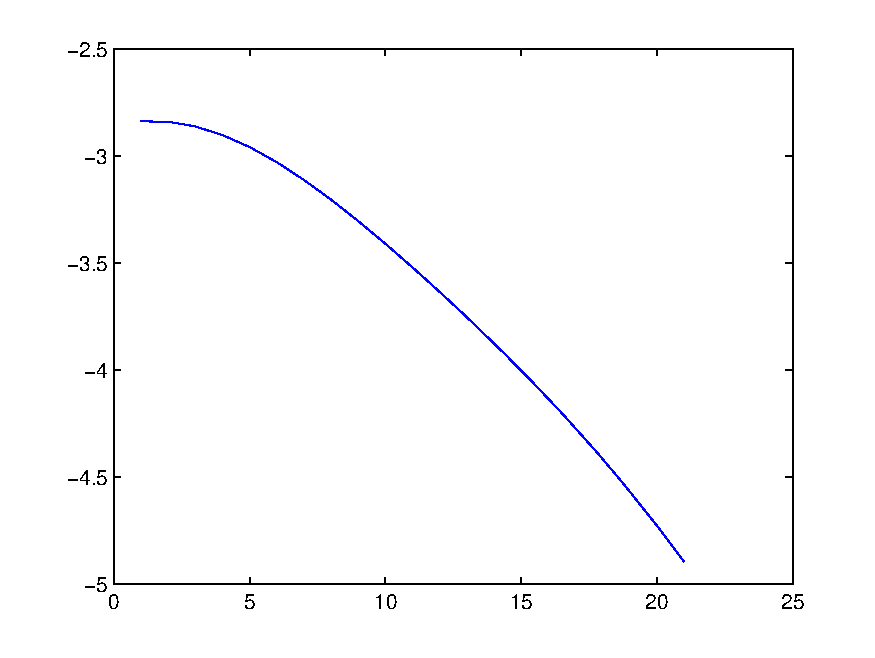
\includegraphics[scale=0.45]{TMPOS.pdf}%width=6cm, height=4cm
\caption{Region of \texttt{TBPOS} around 650 msec.}\label{fig:TMPOS}
\end{wrapfigure}


Given the sample range that includes the actual local maximum (Figure \ref{fig:locmax}), the maximum position in y-dimension can be calculated in the way shown in the following code. First, a vector \texttt{rng} is created containing all sample indices in the range from 250 to 270. All corresponding y-values (second column) in the range \texttt{rng} have been index and assigned to the vector \texttt{y}. The \texttt{max} function in the next line searches for the largest y-value in the vector \texttt{y}. Two output arguments have been returned by the \texttt{max} function -- the maximum positional value \texttt{val} and its index \texttt{idx} of the maximum value in the argument values, i.e., not in the entire signal. We are interested in the second output argument \texttt{idx} that can only be extracted by also calling the first output argument. Multiple output arguments are assigned to variables by combining these with squared brackets \texttt{[]}. The local index of the maximum value \texttt{idx} has been given as index to the vector \texttt{rng} to get the relevant sample value of the signal that corresponds to the maximum y-value, which is assigned to \texttt{idx\_new}. Given the sample index of the file, the time stamp of the local maximum can be calculated by subtracting 1 from the sample value (see Section \ref{spasig}), divided over the sampling rate to get the duration as in equation \eqref{eq:t} in Section \ref{spasig}, multiplying it by 1000 for msec. We thus find that the local maximum of the y-value in \texttt{TBPOS} occurs at 647.50 msec.

\begin{verbatim}
>> rng = 250:270

rng =

  Columns 1 through 16

   250   251   252   253   254   255   256   257   258   259   [...]

  Columns 17 through 21

   266   267   268   269   270
   
>> y = data(2).SIGNAL(rng,2)

y =

    1.5934
    1.6134
    1.6427
    1.6794
...

>> [val idx] = max(y)

val =

    1.8798

idx =

    11

>> idx_new = rng(idx)

idx_new =

   260

>> maxms = 1000*(idx_new-1)/data(2).SRATE

maxms =

  647.5000
\end{verbatim}

The region of interest defined above including the relevant time stamp in samples can also be applied to other trajectories. All trajectory fields and the audio field are synchronous in terms of samples. The trajectory \texttt{TMPOS} can be accessed by changing the field to 3 as in the code below. The same sample region as for the trajectory \texttt{TBPOS} in Figure \ref{fig:locmax} is shown in Figure \ref{fig:TMPOS} for the \texttt{TMPOS} trajectory, which shows different spatial configurations for different sensors at the same point in time.


\begin{verbatim}
>> plot(data(3).SIGNAL(250:270,2))
\end{verbatim}

\subsection{Velocity signals}\label{velsign}

Now we come to the calculation of the vertical, horizontal, and tangential velocity as exemplified in the code below. Velocity values are sometimes predefined for some fields. If so this is usually seen in the field name, which should have an \texttt{\_vel} extension. However, we will show for \texttt{TBPOS} how to calculate velocity values. Feel free to calculate the velocity for other trajectories. First, the signal values of \texttt{TBPOS} are assigned to \texttt{s}. The following formula computes the velocity and stores it in the vector \texttt{vel}. The formula differentiates the positional signals using the so-called \textit{central difference approximation} for the calculation of the derivative.  This calculation is done on the basis of samples. To go from \texttt{vel} to the individual dimension velocities (x, y) expressed in centimeters per second (cm/sec)  we proceed as follows. We need to convert from samples to secs and from millimeters (mm) to cm. For the first conversion, the signal needs to be multiplied with the sampling rate of the trajectory \texttt{SRATE}, according to equation \eqref{eq:s} in Section \ref{spasig}. For the second conversion, in all formulas, we must divide by 10 (\texttt{./} below means that every cell entry in the array will be divided by 10) for the unit conversion from mm to cm (1 cm = 10 mm), so the resulting velocity values are in the usual cm per second units. The vertical velocity can be appended to the array of \texttt{TBPOS} (i.e., \texttt{data(2)}) by defining a new field in it (here, \texttt{VEL\_y}). Note that only the second column of \texttt{vel} is used, since the vertical velocity corresponds to the y-value. The same can be done for the horizontal velocity which is shown in the line after using only using the x-values in the first column. 

\begin{verbatim}
>> s = data(2).SIGNAL;
>> vel = [diff(s(1:2,:)) ; s(3:end,:) - s(1:end-2,:) ; diff(s(end-1:end,:))] ./ 2;
>> data(2).VEL_y =  data(2).SRATE*vel(:,2)./10; 
>> data(2).VEL_x =  data(2).SRATE*vel(:,1)./10;
\end{verbatim}

The tangential velocity (also known as resultant velocity) is defined as the square root of the sum of the squared velocities in each dimension (see equation \eqref{eq:tv}). Following this equation, we can compute the tangential velocity using the command below and appended it to \texttt{data(2)} in the field \texttt{VEL\_tang}, again after multiplying by sampling rate according to equation \eqref{eq:s} in Section \ref{spasig} and dividing by 10 for cm per second velocity units. \texttt{data(2)} shows the three new fields we have just appended to the \texttt{TBPOS} corresponding to the different velocities.

\begin{equation}
v_t = \sqrt{v_{x} ^ 2 + v_{y} ^ 2} \label{eq:tv}
\end{equation}



\begin{verbatim}
>> v_t = sqrt(sum(vel.^2,2));

>> data(2).VEL_tang = data(2).SRATE*v_t./10; 

data(2)

ans = 

      SIGNAL: [928x2 double]
       SRATE: 400
        NAME: 'TBPOS'
       VEL_y: [928x1 double]
       VEL_x: [928x1 double]
    VEL_tang: [928x1 double]
\end{verbatim}


\noindent\textbf{Exercise 7:} Plot the tangential velocity of \texttt{TBPOS} in the region that has been used for the local maximum (250 to 270). Also, determine the corresponding local minimum of the tangential velocity. This minimum corresponds to what labeling software of articulatory kinematics considers to be a maximum constriction. You basically will have to change the field \texttt{SIGNAL} to \texttt{VEL\_tang}. Then, calculate the minimum by applying the function \texttt{min} instead of \texttt{max} (use the \texttt{help} function for \texttt{min}). You might see that the given range does not include a local minimum (cf.\,Figure \ref{fig:locmax} and \ref{fig:increase} in Section \ref{locext}). In this case, increase the range and re-plot. If you follow the detection of the local maximum, this exercise can be solved easily.\par\smallskip


\subsection{Relating spatial and velocity signals}\label{relSpaVelSig}

We have seen that in each file one time stamp or sample index has corresponding spatial values in different signals. Signals can be expressed as spatial in the x-\,and y-dimension or as velocity in a particular dimension and as tangential velocity. Like introduced in the formula in the previous Section \ref{velsign}, we first assign the signal \texttt{TBPOS} to a variable \texttt{s} for an easier handling and its velocity in terms of samples to \texttt{vel}. For now, we keep both signal and velocity in the samples unit.


\begin{verbatim}
>> s = data(2).SIGNAL;
>> vel = [diff(s(1:2,:)) ; s(3:end,:) - s(1:end-2,:) ; diff(s(end-1:end,:))] ./ 2;
\end{verbatim}

\setlength\intextsep{-10pt}
\begin{wrapfigure}[10]{o}{6.3cm}
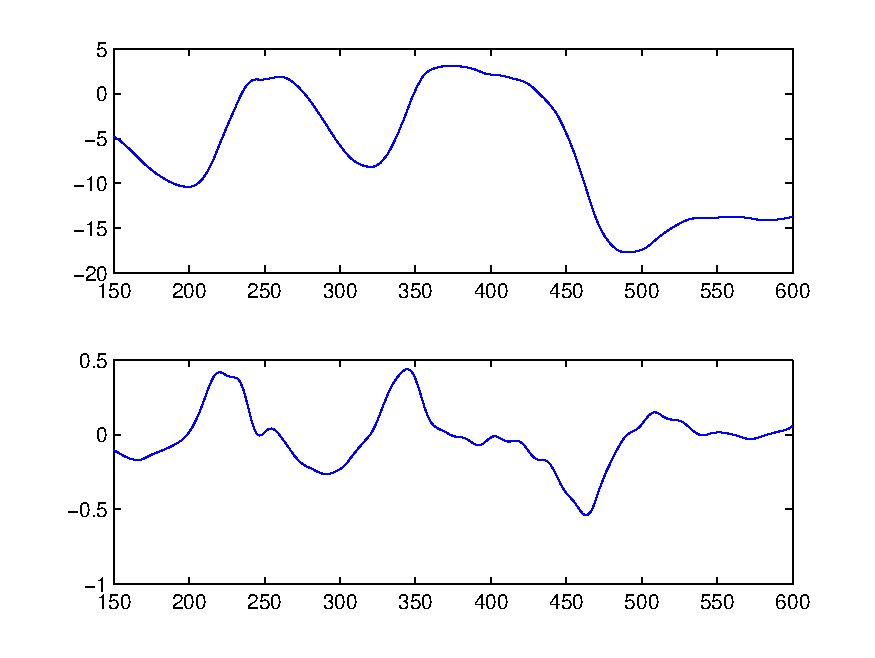
\includegraphics[scale=0.45]{ysign.pdf}%width=6cm, height=4cm
\caption{Vertical movement (upper panel) and vertical velocity (lower panel) of \texttt{TBPOS}.}\label{fig:yvel}
\end{wrapfigure}

Since we want to plot different signals independently in a comparable fashion the \texttt{subplot} command is introduced below. To illustrate the correspondence between particular time slices and different signals, the following command plots different signal types of \texttt{TBPOS} in the sample range from 150 to 600. Using \texttt{figure(1)} a figure object is created. The command \texttt{subplot} takes here three arguments. The first determines the number of rows of the output figure and the second the number of columns, such that a 2$\times$1 plot is produced. The last number in \texttt{subplot} specifies the position of the plot. The plots are specified after the comma. For both the signal \texttt{s} and the velocity \texttt{vel}, the y-signal, i.e.\,the vertical spatial signal and the vertical velocity, is index by \texttt{2} for the range between 150 and 600. Thus both vertical signals correspond to the same range in the same trajectory (i.e., \texttt{TBPOS}). In the first argument of both plots, the sample range is specified. The output is shown in Figure \ref{fig:yvel}. By default, MATLAB aligns the x-axis starting with 0 (try out, and remove the first argument of the \texttt{plot} functions). The upper panel of Figure \ref{fig:yvel} shows the vertical movement of \texttt{TBPOS}. The vertical velocity shown in the lower panel corresponds to the vertical movement. At approximately 380 samples a positive peak in the positional signal (upper panel) is surrounded by a two extrema in the velocity signal (lower panel) with one positive extremum and the other negative and in between the two extrema the velocity cross zero. You can close the open figure by typing \texttt{close all} in you MATLAB console.\par

\begin{verbatim}
>> figure(1)
>> subplot(2,1,1), plot(150:600, s(150:600,2))
>> subplot(2,1,2), plot(150:600, vel(150:600,2))
\end{verbatim}


The same code as for the vertical signals in Figure \ref{fig:yvel} can be applied to the horizontal signal by changing the column index to \texttt{1} which corresponds to the x-values as shown below. Note, the range of the signal is still the same, such as the trajectory. Now, the signal corresponds to the movement in the horizontal dimension. Figure \ref{fig:xvel} shows the output plot. Again, the upper panel shows the spatial movement in the horizontal dimension, and the lower panel shows the corresponding velocity.

\begin{verbatim}
>> figure(2)
>> subplot(2,1,1), plot(150:600, s(150:600,1))
>> subplot(2,1,2), plot(150:600, vel(150:600,1))
\end{verbatim}

\setlength\intextsep{-10pt}
\begin{wrapfigure}[10]{o}{6.3cm}
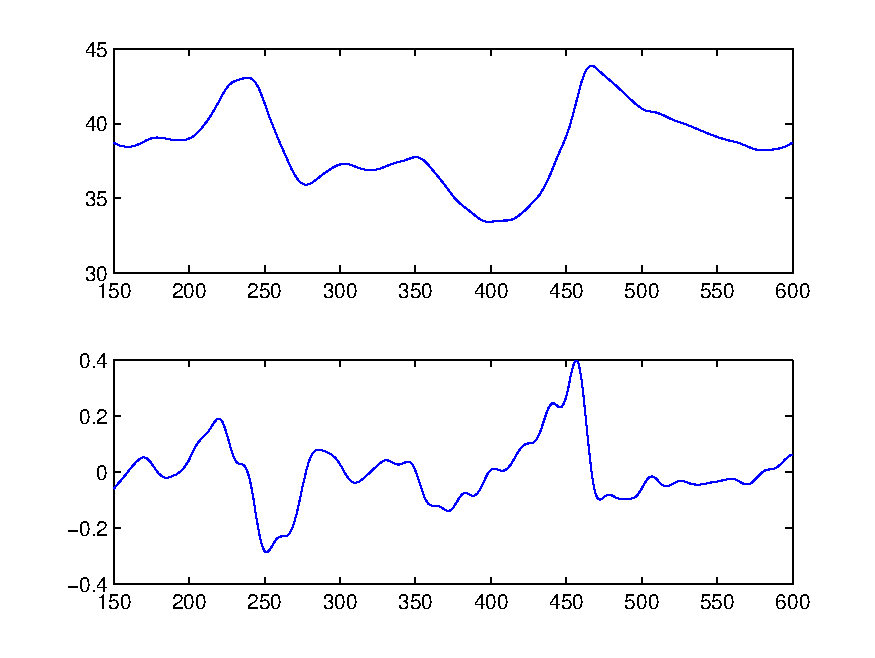
\includegraphics[scale=0.45]{xsign.pdf}%width=6cm, height=4cm
\caption{Horizontal movement (upper panel) and horizontal velocity (lower panel) of \texttt{TBPOS}.}\label{fig:xvel}
\end{wrapfigure}

\noindent\textbf{Exercise 8:} Create the similar plots like in Figure \ref{fig:yvel} and in Figure \ref{fig:xvel} for \texttt{TMPOS} in the sample range from 550 to 650. Observe the sensitivity to local extrema under the variation of the sample range. Vary the sample between (e.g., 200 to 700, 300 to 500, 400 to 450). You will have to change to index of the signal \texttt{s} assignment and the range values. Hint: You can save yourself some work, by creating a vector, say \texttt{range}, that contains the sample slice of interest.\par\smallskip



In Figure \ref{fig:yvel} and Figure \ref{fig:xvel}, we are still in the realm of spatial movement and velocities in sample coordinates for the x-axis. In the code below, the velocity values will be converted to cm/sec similar to the conversion shown in Section \ref{velsign}. The tangential velocity is computed as shown in equation \eqref{eq:tv} in Section \ref{velsign} and assigned to \texttt{t}. All three velocities are multiplied by its sampling rate as in equation \eqref{eq:s} in Section \ref{spasig} and divided by 10 for cm/sec. The sampling rate of the respective trajectory \texttt{TBPOS} was assigned to \texttt{sRate}. 

\begin{verbatim}
>> sRate = data(2).SRATE;
>> yvel =  sRate*vel(:,2)./10; 
>> xvel =  sRate*vel(:,1)./10;
>> t = sqrt(sum(vel.^2,2));
>> tvel = sRate*t./10; 
\end{verbatim}

Additionally, the x-axis in the plots should be in a time unit (msec). In the code below the sample sequence that we are interested in is assigned to \texttt{range} for convenience. A time vector \texttt{ms\_unit} is created with \texttt{linspace} similar to the example shown in Section \ref{spasig}. Given the vector \texttt{range} it is easier to change the range later on and re-plot the figures without changing the sample slice in each line. Some changes in the \texttt{linspace} command must be pointed out: The first argument, which is the beginning of the spaced vector is the first element in range index by \texttt{1}. This value is divided by the sampling rate \texttt{sRate} for seconds as in equation \eqref{eq:t} in Section \ref{spasig}. The second argument is the end of the spaced vector specified by the final index in \texttt{range} using \texttt{end} which returns the last value. The length of the vector \texttt{range} is provided as last argument. The results are multiplied with 1000 for msec and assigned to \texttt{ms\_unit}.

\begin{verbatim}
>> range = 150:600;
>> ms_unit = 1000*(linspace(range(1)/sRate, range(end)/sRate, length(range)));
\end{verbatim}

\setlength\intextsep{-10pt}
\begin{wrapfigure}[10]{r}{6.3cm}
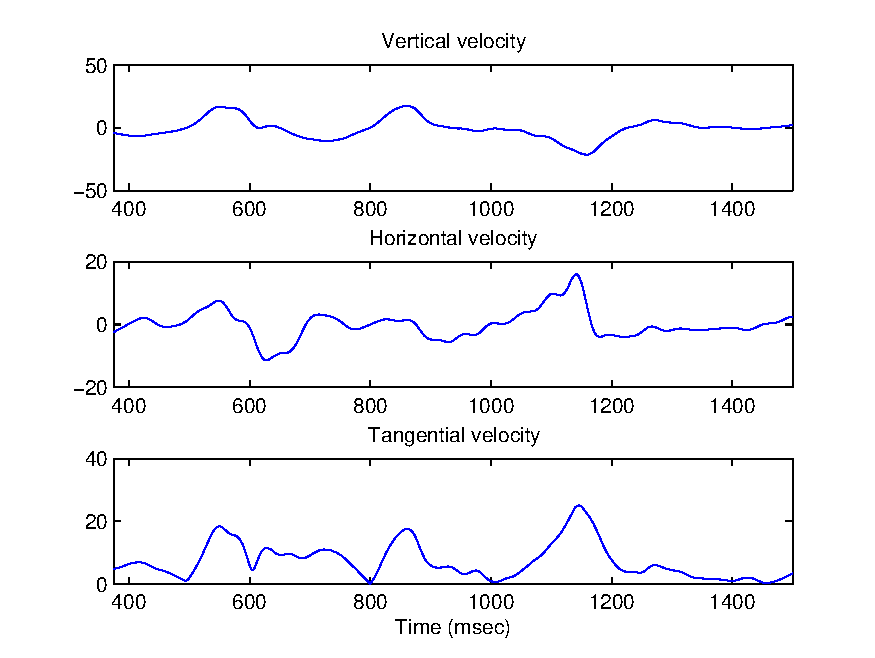
\includegraphics[scale=0.45]{velms.pdf}%width=6cm, height=4cm
\caption{Vertical velocity (upper panel), horizontal velocity (middle panel), and tangential velocity (lower panel) of \texttt{TBPOS}.}\label{fig:velms}
\end{wrapfigure}


Figures with the different velocity types can now be created in the code below, introducing a new figure with \texttt{figure(3)} and creating a 3$\times$1 subplot like described above. The time vector \texttt{ms\_unit} created above is the first argument in the \texttt{plot} function and determines the values of the x-axis. Since we saved the sequence of interest in the vector \texttt{range}, it can be applied to each of the velocity vectors (i.e., \texttt{yvel}, \texttt{xvel}, and \texttt{tvel}). This manner makes it easier to change the range for new plots. The limits of the x-axis have been defined for each plot using \texttt{xlim} which takes a matrix indicated by the squared brackets that contains the limits, though the beginning (i.e., \texttt{ms\_unit(1)}) and the end of the x-axis (i.e., \texttt{ms\_unit(end)}). Titles for each plot are added using the \texttt{title} function which takes a string as argument being the title. The x-label can be added using the \texttt{xlabel} function which takes a string that specifies the name of the x-axis. Figure \ref{fig:velms} shows the returned plot with the vertical velocity in the upper panel, the horizontal velocity in the middle panel, and the tangential velocity in the lower panel. We have looked at the vertical and horizontal velocity before. When it comes to the tangential velocity, both extrema are positive and in between the extrema the velocity dips to a value close to zero (but not necessarily zero; it is never negative though since the tangential velocity entails the squared vertical and horizontal velocities). For instance, we find a positive extremum for the vertical velocity (upper panel) at approximately 800 msec that corresponds to a positive peak in the tangential velocity (lower panel). The zero crossing in the vertical velocity at approximately 1000 msec shows a peak in local minimum in the tangential velocity and the negative extremum in vertical velocity peaks at 1200 msec, which corresponds to a maximum peak in tangential velocity. 


\begin{verbatim}
>> figure(3)
>> subplot(3,1,1), plot(ms_unit, yvel(range))
>> xlim([ms_unit(1), ms_unit(end)])
>> title('Vertical velocity')
>> subplot(3,1,2), plot(ms_unit, xvel(range))
>> xlim([ms_unit(1), ms_unit(end)])
>> title('Horizontal velocity')
>> subplot(3,1,3), plot(ms_unit, tvel(range))
>> xlim([ms_unit(1), ms_unit(end)])
>> title('Tangential velocity')
>> xlim([ms_unit(1), ms_unit(end)])
>> xlabel('Time (msec)')
\end{verbatim}





\noindent\textbf{Exercise 9:} Repeat Exercise 8 for the different velocity signals of the code for Figure \ref{fig:velms}. Use \texttt{TMPOS} and the time slices in Exercise 8, compute the velocity signals in cm/sec and change the x-axis to msec. Re-plot \texttt{figure(3)} for different time slices determined in a vector \texttt{range}.\par\smallskip


\subsection{Storing labels}\label{storlab}

Having extracted a time stamp from a trajectory, the relevant information can be stored in a new structure array that will be called \texttt{labels}. The code below shows how to store information in a new structure array. For the first entry in the new structure array, \texttt{labels} must be indexed with \texttt{1}. This new structure array has its own fields that you as the researcher will find useful. These field names are specified subsequently of \texttt{labels(1)} using a dot. You can have as many fields as you find useful. As fields for our structure here, we will use names that are mnemonic of the information we extracted in the example task in Section \ref{locext}. For instance, the field \texttt{file} stores the name of the file that has been stored in the variable \texttt{names} (Section \ref{sec:emastruc}) or can be assigned directly as a string \texttt{`cascade\_09\_0823'}.

\begin{verbatim}
>> labels(1).file = names{1};
>> labels(1).trajectory = trajectories{2};
>> labels(1).name = 'MAX_C';
>> labels(1).timestamp = maxms;
>> labels(1).signal = 'y';
>> labels(1).phone = 'a'

labels = 

          file: 'cascade_09_0823'
    trajectory: 'TBPOS'
          name: 'MAX_C'
     timestamp: 647.5000
        signal: 'y'
         phone: 'a'
\end{verbatim}
 
The output shows the information that we have assigned to the structure array, e.g., the file name, the trajectory, the name of the landmark, the time stamp etcetera.

If a new hypothetical value is to be appended to the same structure array, increase the index to the next value. In the case below, we use \texttt{2}, but if you are not aware of how many values are contained in a structure array you can name the index \texttt{end}. This appends the new information to the end of the structure array. As you will see in the output (type \texttt{labels}), the structure array has now the size 1$\times$2, since we have added one information point.\par

\begin{verbatim}
>> labels(2).file = names{1};
>> labels(2).trajectory = trajectories{2};
>> labels(2).name = 'MAX_C';
>> labels(2).timestamp = 652.5;
>> labels(2).signal = 'x';
>> labels(2).phone = 'a'

labels = 

1x2 struct array with fields:
    file
    trajectory
    name
    timestamp
    signal
    phone
\end{verbatim}

If you are interested in the information that you have just stored in the structure array, it can be accessed with the index \texttt{2} like shown below. Also, you can access only particular information like the label's name by adding the field \texttt{name} to the index structure array (e.g., \texttt{labels(2)}).

\begin{verbatim}
>> labels(2)

ans = 

          file: 'cascade_09_0823'
    trajectory: 'TBPOS'
          name: 'MAX_C'
     timestamp: 652.5000
        signal: 'tang vel'
         phone: 'a'
         
>> labels(2).name

ans =

MAX_C         
\end{verbatim}


\noindent\textbf{Exercise 10:} Given the results that you gained from Exercise 7, append your information to the structure array \texttt{labels}. Use \texttt{end} instead of increasing the index of \texttt{labels} as described in text above. The value for the field name \texttt{signal} must be something like \texttt{vel\_tang} (i.e., tangential velocity) and obviously the value for the field \texttt{timestamp} is the time stamp that you determined in Exercise 7. If you are done with this, type \texttt{labels} in the MATLAB console, and a 1$\times$3 structure array should be returned.\par\smallskip

\section{Landmark finder}

This section describes an algorithm which delimits an interval over the movement trace of an EMA receiver coil using kinematic quantities measured on the trace (Section~\ref{subsec:oneMT}). The algorithm is straightforward to scale up to delimit intervals over a set of movement traces (Section~\ref{subsec:mtSet}).

\subsection{Finding landmarks on one movement trace}
\label{subsec:oneMT}

Commonly we are interested in a vocal tract event and its record in the movement trace of an EMA receiver coil. The goal of an analysis might then be to find the time interval over which the event unfolds in the EMA record. This section presents an algorithm to find landmarks in the movement trace of an EMA receiver coil which index the beginning and end of this interval as well as other important time points as the event unfolds in time.\footnote{The MATLAB demo file is landmark\_finder\_main.m in the directory util.}

Among the time points which we seek is the left edge of the interval, which marks the beginning of the interval of interest, as well as the right edge of the interval, which marks the end of this interval. We consider the case where this event is centered on a maximum in the velocity signal, i.e. we seek an interval over which a single articulator undergoes displacement, and so we also seek to find the time point of peak velocity.

Let us examine the EMA record of the production of the word ``bulha'' embedded in the carrier phrase ``jibi \_\_\_ hnaya'', and in particular let us examine the movement trace of the tongue tip receiver coil during the alveolar constriction of \textipa{/l/}. Our goal is to delimit an interval over which this alveolar constriction unfolds. We begin by declaring a few constants
\begin{verbatim}
fileName = 'bulha_01_0005.mat';
articulator = 'TTIPPOS';
\end{verbatim}
and by loading in the .mat file for analysis. 
\begin{verbatim}
S = load(fileName);
tokenName = fileName(1:end-4);
S = S.(tokenName);
\end{verbatim}
The object \texttt{S} is the structure array which is by now the familiar container data structure for the experimentally recorded time series. We assign the two dimensional movement trace (a $500\times 2$ matrix) to the variable \texttt{x}.
\begin{verbatim}
x = S(strmatch(articulator,{S.NAME})).SIGNAL;
\end{verbatim}
The sampling rates of the EMA and audio recordings are assigned to variables.
\begin{verbatim}
srate = S(strmatch(articulator,{S.NAME})).SRATE;
audioSrate = S(strmatch('audio',{S.NAME})).SRATE;
\end{verbatim}
We assign the vector of sampling time points in milliseconds to the variable \texttt{t}.
\begin{verbatim}
t = sampl2ms(1:length(x),srate);
\end{verbatim}
Finally, we assign the tangential velocity of the receiver coil to the variable \texttt{x\_t}. Throughout this section we adopt the convention that \texttt{x\_t} denotes differentiation of \texttt{x} with respect to time \texttt{t}. The units of \texttt{x\_t} are cm/sec. By using the function \texttt{derivative(x)} we average neighboring values of the finite differences \texttt{diff(x)} in order to obtain a vector estimate of the tangential velocity record which preserves the length of \texttt{x}. So \texttt{x\_t} is a vector of length 500.
\begin{verbatim}
x_t = srate .* sqrt(sum(derivative(x).^2,2)) ./ 10;
\end{verbatim}

We use a built-in MATLAB graphical user interface (GUI) in order to interactively identify a rough guess at the time point of peak velocity of interest. The following is a wrapper function \texttt{plotGUI} which prepares a graphical display on figure panel one which the human user will interact with.
\begin{verbatim}
function plotGUI(S,t,x,x_t,articulator,srate,audioSrate,vargin)
    % PLOTGUI - plot the position and velocity of the articulator
    % trajectory.
    
    if nargin == 7 || nargin == 8
        figure(1);
        subplot(3,1,1)
        audio = S(1).SIGNAL;
        audioT = sampl2ms(1:length(audio),audioSrate);
        plot(audioT,audio);
        title(articulator); 
        subplot(3,1,2)
        plot(t,x(:,1)-mean(x(:,1)),'Color',[.8,.3,.3],'LineWidth',2), hold on
        plot(t,x(:,2)-mean(x(:,2)),'Color',[.3,.8,.3],'LineWidth',2);
        ylabel('x-red, y-green (mm)'),xlabel('time (msec)'),hold off
        subplot(3,1,3)
        plot(t,x_t,'LineWidth',2), hold on
        ylabel('tangential velocity (cm/sec)'),xlabel('time (msec)')
    else
        error('Error: plotGUI is not called correctly.');
    end
    
    if nargin == 8
        [le,lev,tpv,pv,re,rev,~,vp] = deal(vargin{:});
        projT = le+sampl2ms(1:length(vp),srate).';
        plot(projT,vp,'Color',[0.8,0.2,0.2],'LineWidth',2);
        scatter(le,lev,[],[0.9,0.2,0.2],'filled'); 
        scatter(tpv,pv,[],[0.2,0.9,0.2],'filled'); 
        scatter(re,rev,[],[0.2,0.2,0.9],'filled');
    end
    hold off
end
\end{verbatim}
The function \texttt{plotGUI} prepares a graphical display with three panels stacked one on top of the other. The top panel is the acoustic waveform, the middle panel is the plot of the two dimensional tongue tip movement trace over the whole EMA record. The horizontal (anterior-posterior) position is plotted red and the vertical (superior-inferior) position is plotted green. We center these records about zero for the purpose of graphical display. The tangential velocity is plotted in the bottom panel. See figure~\ref{fig:gui}. 
\begin{figure}
\centering
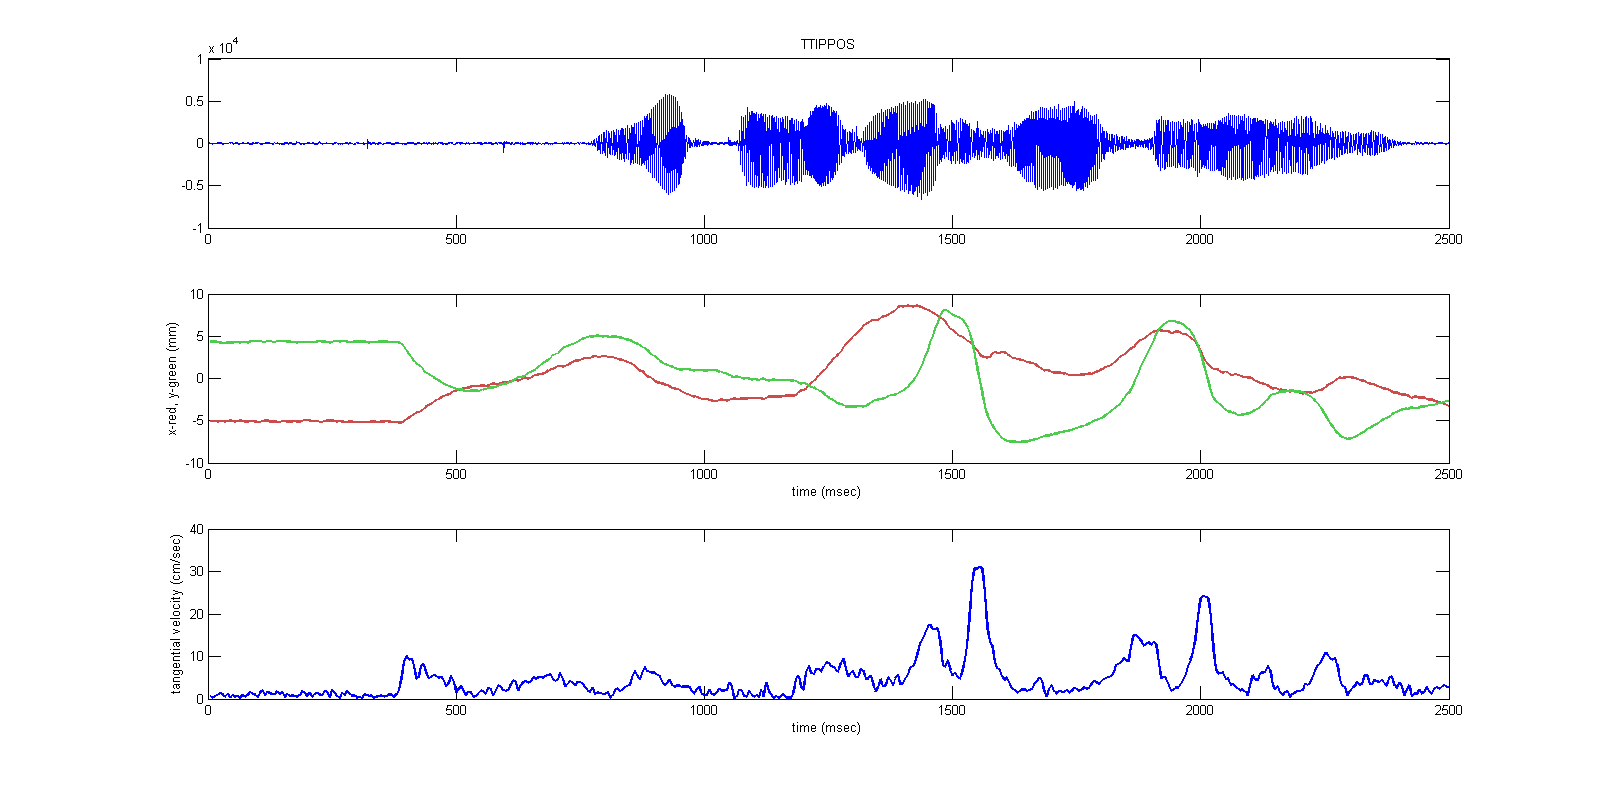
\includegraphics[width=.8\textwidth]{p1.png}
\caption{The graphical user interface (GUI) used by the user-defined function \texttt{plotGUI}.}
\label{fig:gui}
\end{figure}
The following code prepares the graphical display with \texttt{plotGUI}, calls MATLAB's built-in GUI input function \texttt{ginput} on figure~\ref{fig:gui}, and waits until the user clicks on the peak velocity of interest in the bottom panel of figure~\ref{fig:gui}.
\begin{verbatim}
% Plot signal and resultant velocity.
plotGUI(S,t,x,x_t,articulator,srate,audioSrate)

% User input of guess TPVGUESS of the time of peak velocity TPV.
[tpvGuess,~] = ginput(1); iter = 1; skip = 0;
while (~isempty(tpvGuess) || iter == 1) && ~skip
    
    % Find landmarks.
    [le,lev,tpv,pv,re,rev,u,hook,vp,disp,lambda] = findLandmarks(x, ...
        srate, tpvGuess, {.1,10,.8,'threshold','pcaProj',150});
    
    % User input. If correct, press ENTER. If you want to redo, guess 
    % again.
    plotGUI(S,t,x,x_t,articulator,srate,audioSrate,{le,lev,tpv,pv,re,rev,u,vp})
    redo = input('redo? [1] ');
    if ~isempty(redo), [tpvGuess,~] = ginput(1); else tpvGuess = []; end
    
    iter = iter+1;
end
cla
\end{verbatim}
The GUI records the y-coordinate of the point under the cursor in figure~\ref{fig:crosshairs}. The y-coordinate of our cursor position is near the peak velocity of the tongue tip movement trace on its way toward the alveolar ridge. 
\begin{figure}
\centering
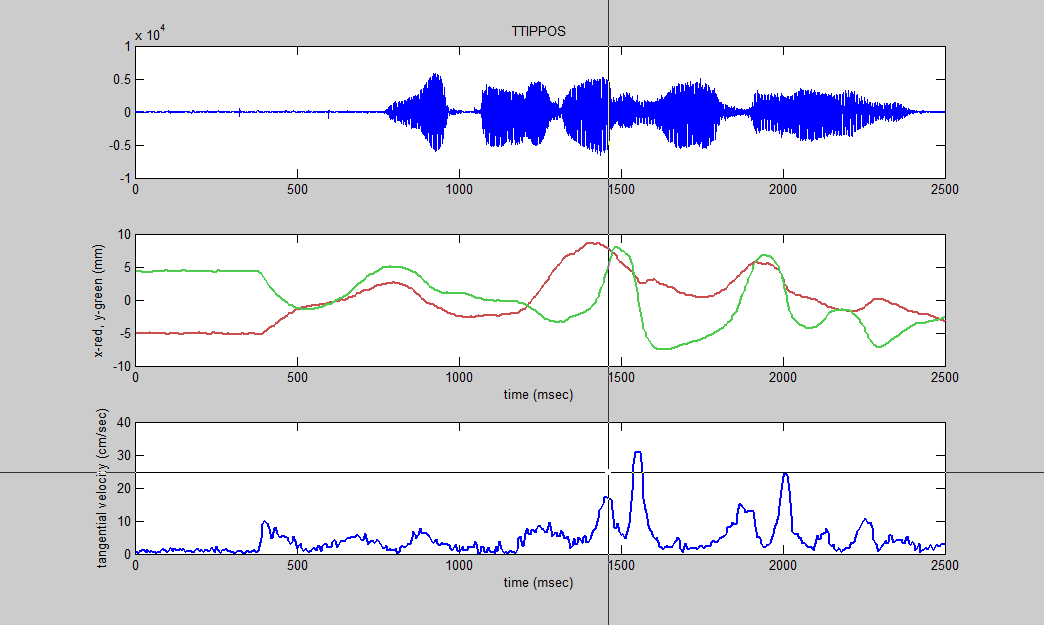
\includegraphics[width=.8\textwidth]{p2.png}
\caption{The cursor is at a point whose y-coordinate is near the peak velocity of interest in the GUI.}
\label{fig:crosshairs}
\end{figure}
Once the user clicks on the peak velocity of interest, the algorithm \texttt{findLandmarks} is passed the time point at which the user clicked, which has been assigned to the variable \texttt{tpvGuess}. The function \texttt{findLandmarks} finds the sample at which the nearest velocity peak occurs and delimits the y-coordinate where the user clicks. The estimated landmarks can be confirmed by pressing enter (or return) once. Otherwise, pressing the number one and then enter (or return) allows the user a redo. We now step through this algorithm step by step. It begins by converting \texttt{tpvGuess} from milliseconds to samples and by declaring some variables.
\begin{verbatim}
function [le,lev,tpv,pv,re,rev,u,hook,vp,disp,lambda] = findLandmarks(x, ...
        srate, tpvGuess, vargin)
% findLandmarks - find sample at which peak velocity occurs and delimit the
% left and right edges of an interval.

tpvGuess = ms2sampl(tpvGuess,srate);
u = [];
\end{verbatim}
The fourth argument to \texttt{findLandmarks} specifies that the movement trace of the tongue tip receiver coil \texttt{x} is to be projected down onto one dimension. 
We first impose a change of coordinates system on the data by finding the principal component \texttt{u} of movement and its orthogonal complement. 
We do this by finding the covariance matrix of the matrix \texttt{x}, which contains the two dimensional movement trace, over a time window whose length \texttt{pcaWin} is given in milliseconds. We find the eigenvalues of this covariance matrix and the associated eigenvectors. The eigenvector whose eigenvalue is the greater of the two is the principal component \texttt{u}. The other vector is its orthogonal complement. These two vectors are the basis of the new coordinate system. We project \texttt{x} onto \texttt{u}, whose eigenvalue was the greater of the two. The variable \texttt{x} has now been redeclared as a vector containing the original movement trace projected onto \texttt{u}. See figure~\ref{fig:projection} for a graphical illustration of the two dimensional movement trace, its principal component \texttt{u}, and the movement trace projected onto \texttt{u}.
\begin{verbatim}
if strcmp(preproc,'pcaProj')
    [x,u,lambda] = pcaProj(x,tpvGuess,srate,pcaWin);
else
    lambda = [];
end
\end{verbatim}
\begin{figure}
\centering
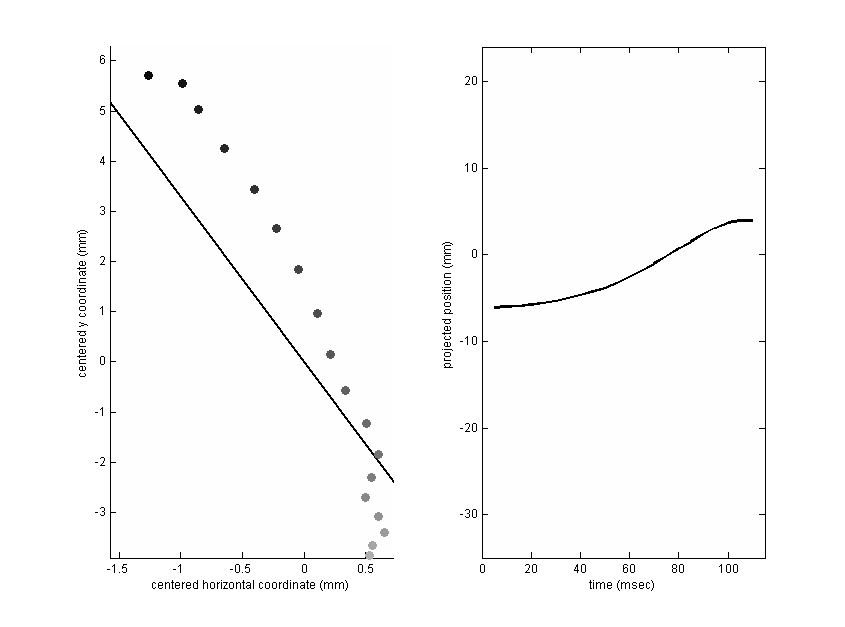
\includegraphics[width=.8\textwidth]{p5.png}
\caption{The tongue body movement trace \texttt{x} in the saggital plane (the grayer the sampled position, the earlier the time point) and the line passing through the principal component \texttt{u} and the origin (left panel). The movement trace \texttt{x} is projected onto the principal component \texttt{u}, and the projected movement trace is plotted against time (right panel).}
\label{fig:projection}
\end{figure}

Principal components analysis (PCA) is a common statistical method for the analysis of high dimensional data, but here we use it to identify a change of basis for a two dimensional data set which yields a meaningful axis along which to analyze an alveolar constriction. For an application of PCA to a high dimensional problem in phonetics, see~\citet{story2007}. For an application in movement science more broadly construed, see~\citet{tseng2003}. For discussion of its use (and an alternative) in analyzing high dimensional data sets more generally, see~\citet{schoener2007}.

The movement trace \texttt{x} is now one dimensional. We approximate the derivative of \texttt{x} by the finite difference method to obtain the velocity profile of the movement trace along \texttt{u}.
\begin{verbatim}
x_t = sqrt(sum(derivative(x).^2,2));
\end{verbatim}
At this point it is useful to filter the velocity profile to obtain a signal which is less likely to have spurious local maxima and minima. We choose a moving average filter. The value of the filtered velocity profile at a point $p$ is determined by the average of all the values of the points within a window, which is \texttt{fWin} samples long, surrounding $p$.
\begin{verbatim}
fx_t = filtfilt(ones(1,fWin)./fWin,1,x_t);
\end{verbatim}
The time point of the maximum of the filtered velocity profile \texttt{fx\_t} is a useful approximation to the time point of peak velocity in \texttt{x\_t}. However, the moving average filter does not provide a good approximation to the magnitude of peak velocity. This can be seen by comparing the filtered velocity profile in red to the unfiltered velocity profile in blue. See figure~\ref{fig:filter}. When using a moving average filter, then, it is important to keep these observations in mind.
\begin{figure}
\centering
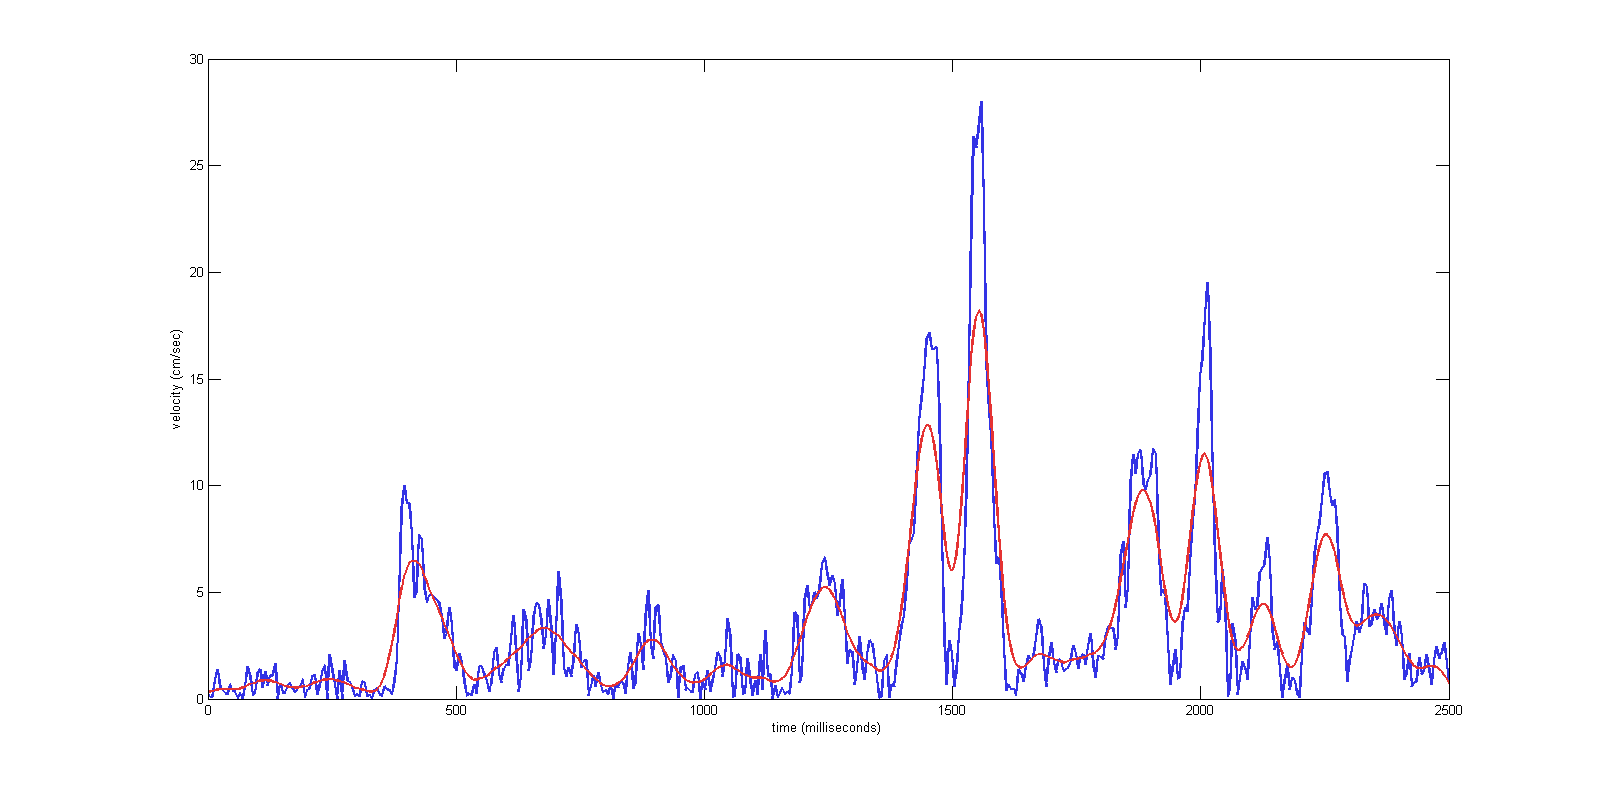
\includegraphics[width=.8\textwidth]{p4.png}
\caption{The filtered velocity profile (red) gives a good approximation to the time of peak velocity in the unfiltered velocity profile (blue), but the moving average filter does not give a good approximation to the magnitude of the velocity, especially at maxima and minima.}
\label{fig:filter}
\end{figure}
\begin{verbatim}
[~,pks] = findpeaks(fx_t);
\end{verbatim}
We locate the time point of peak velocity of the filtered velocity profile \texttt{fx\_t} which is closest to our guess which we made on the basis of visual inspection.
\begin{verbatim}
[~,tpvGuess] = min(abs(pks-tpvGuess));
\end{verbatim}
The peak velocity of the filtered signal \texttt{fx\_t} is then assigned to \texttt{pvGuess}
\begin{verbatim}
pvGuess = fx_t(pks(tpvGuess));
\end{verbatim}
and the time of peak velocity of the filtered signal \texttt{fx\_t} is then assigned to \texttt{tpvGuess}.
\begin{verbatim}
tpvGuess = pks(tpvGuess);
\end{verbatim}
Having made good approximations \texttt{pvGuess} and \texttt{tpvGuess} to the peak velocity and time of peak velocity, respectively, we use these refined guesses to locate the peak velocity of the unfiltered velocity profile \texttt{x\_t} nearest to that of the filtered velocity profile \texttt{fx\_t}.
\begin{verbatim}
[~,pks] = findpeaks(x_t);
[~,tpv] = min(abs(pks-tpvGuess));
\end{verbatim}
The variable \texttt{tpv} is the peak velocity of the velocity profile \texttt{x\_t} which is closest to the peak which we found in the filtered signal \texttt{fx\_t}. Before we call this our final estimate of the time of peak velocity, however, we determine whether there are any greater maxima over a 60 millisecond interval around \texttt{pks(tpv)}. If there are, we take the greatest of these local maximima.
\begin{verbatim}
for i = 1:length(pks)
    if abs(pks(tpv)-pks(i)) < ms2sampl(30,srate) && x_t(pks(tpv)) < x_t(pks(i))
        tpv = i;
    end
end
\end{verbatim}
We now have an estimate of peak velocity. The variables \texttt{pv} and \texttt{tpv} are the peak velocity and time of peak velocity, respectively, of \texttt{x\_t}.
\begin{verbatim}
pv = x_t(pks(tpv));
tpv = pks(tpv);
\end{verbatim}

We have now found an estimate of the time of peak velocity and the peak velocity. We use these to delimit a left and right edge to the movement whose peak velocity we have located. Although a speech movement is not discrete, we operationalize the notion of an edge by taking the nearest points at which the velocity rises above and falls below ten percent of the peak velocity as the left and right edges, respectively. This is specified as the fourth element \texttt{'theshold'} of \texttt{vargin}, which we passed to the function \texttt{findLandmarks}, the function which we are describing right now.
\begin{verbatim}
if strcmp(method,'threshold')
    [le,re] = vThreshEdges(fx_t,x_t,tpvGuess,pvGuess,tpv,pv,mphScalar,...
        threshold,fWin);
elseif strcmp(method,'tan')
    [le,re] = vTanEdges(fx_t,x_t,tpvGuess,pvGuess,tpv,pv,mphScalar,fWin);
end
\end{verbatim}
Since we specified that \texttt{method} is \texttt{'threshold'}, the function \texttt{vThreshEdges} is called to delimit the left and right edges of the time interval of interest. We now step through this algorithm. Bear in mind that we are now twice embedded within the call stack.
\begin{verbatim}
function [le,re] = vThreshEdges(fx_t,x_t,tpvGuess,pvGuess,tpv,pv,...
        mphScalar,threshold,fWin)
% VTHRESHEDGES - Find the minima to the left and right of TPV in the 
%   filtered signal. This gives landmarks for the left and right edges 
%   which are unaffected by negligible minima.
\end{verbatim}
We begin by finding the minima around the time \texttt{tpvGuess} of peak velocity of the filtered velocity profile \texttt{fx\_t}.
\begin{verbatim}
[~,leFiltMin] = findpeaks(-wrev(fx_t(1:tpvGuess)),...
        'MINPEAKHEIGHT',-mphScalar.*pvGuess,'NPEAKS',1);
[~,reFiltMin] = findpeaks(-fx_t(tpvGuess:end),...
        'MINPEAKHEIGHT',-mphScalar.*pvGuess,'NPEAKS',1);
\end{verbatim}
We now use these guesses to find the corresponding minima around the time \texttt{tpv} of peak velocity of the unfiltered signal \texttt{x\_t}.
\begin{verbatim}
[leMins,leMinIndices] = findpeaks(-wrev(x_t(1:tpv)));
[reMins,reMinIndices] = findpeaks(-x_t(tpv:end));
[~,leMinIndex] = min(abs(leMinIndices-leFiltMin));
[~,reMinIndex] = min(abs(reMinIndices-reFiltMin));
leMin = -leMins(leMinIndex);
reMin = -reMins(reMinIndex);
\end{verbatim}
It is possible that the minima we found in this way are quite far away from the peak velocity. For this reason we apply a threshold criterion to find the velocity threshold which, when passed on the way rightward or leftward from the peak velocity, indicates that we have reached the right of left edge of the interval of interest.
\begin{verbatim}
leThreshold = leMin + threshold.*(pv-leMin);
reThreshold = reMin + threshold.*(pv-reMin);
\end{verbatim}
These thresholds are applied to find the left and right edges as follows.
\begin{verbatim}
le = find(wrev(x_t(1:tpv))<=leThreshold,1);
le = tpv - le;
re = find(x_t(tpv:end)<=reThreshold,1);
re = tpv + re - 1;

end
\end{verbatim}
We have now found the left and right edges of the interval of interest and exited the function \texttt{vThreshEdges}. Still in the function \texttt{findLandmarks}, we assign the velocity at the left and right edges to the variables \texttt{lev} and \texttt{rev}, respectively. The peak velocity is assigned to \texttt{vp}.
\begin{verbatim}
lev = x_t(le);
rev = x_t(re);
vp = x_t(le:re);
\end{verbatim}
The last thing which \texttt{findLandmarks} does is to convert to the right units.
\begin{verbatim}
le = sampl2ms(le,srate);
tpv = sampl2ms(tpv,srate);
re = sampl2ms(re,srate);
lev = srate .* lev ./ 10;
pv = srate .* pv ./ 10;
rev = srate .* rev ./ 10;
vp = srate .* vp ./ 10;

end
\end{verbatim}

We exit the function \texttt{findLandmarks}. We now have the left and right edges of the interval of interest and the peak velocity around which the interval is centered. We now see that the velocity profile along the principal component \texttt{u} of movement is plotted red in the GUI over the interval from \texttt{le} to \texttt{re}. See figure~\ref{fig:velocityprofile}. This velocity profile is the velocity of the tongue body receiver coil as it moves along the principal component \texttt{u} of its movement on its way to the alveolar ridge for the segment \textipa{/l/}. Bear in mind that although we plot this velocity profile on the same axis, the blue resultant velocity signal and the red velocity profile are the velocity of movement in different subspaces. The blue velocity is the resultant velocity of a two-dimensional movement trace and the red velocity is the velocity along the one-dimensional principal component of the tongue tip movement. For the purpose of graphical display and because the units are the same, however, we plot these on the same panel.
\begin{figure}
\centering
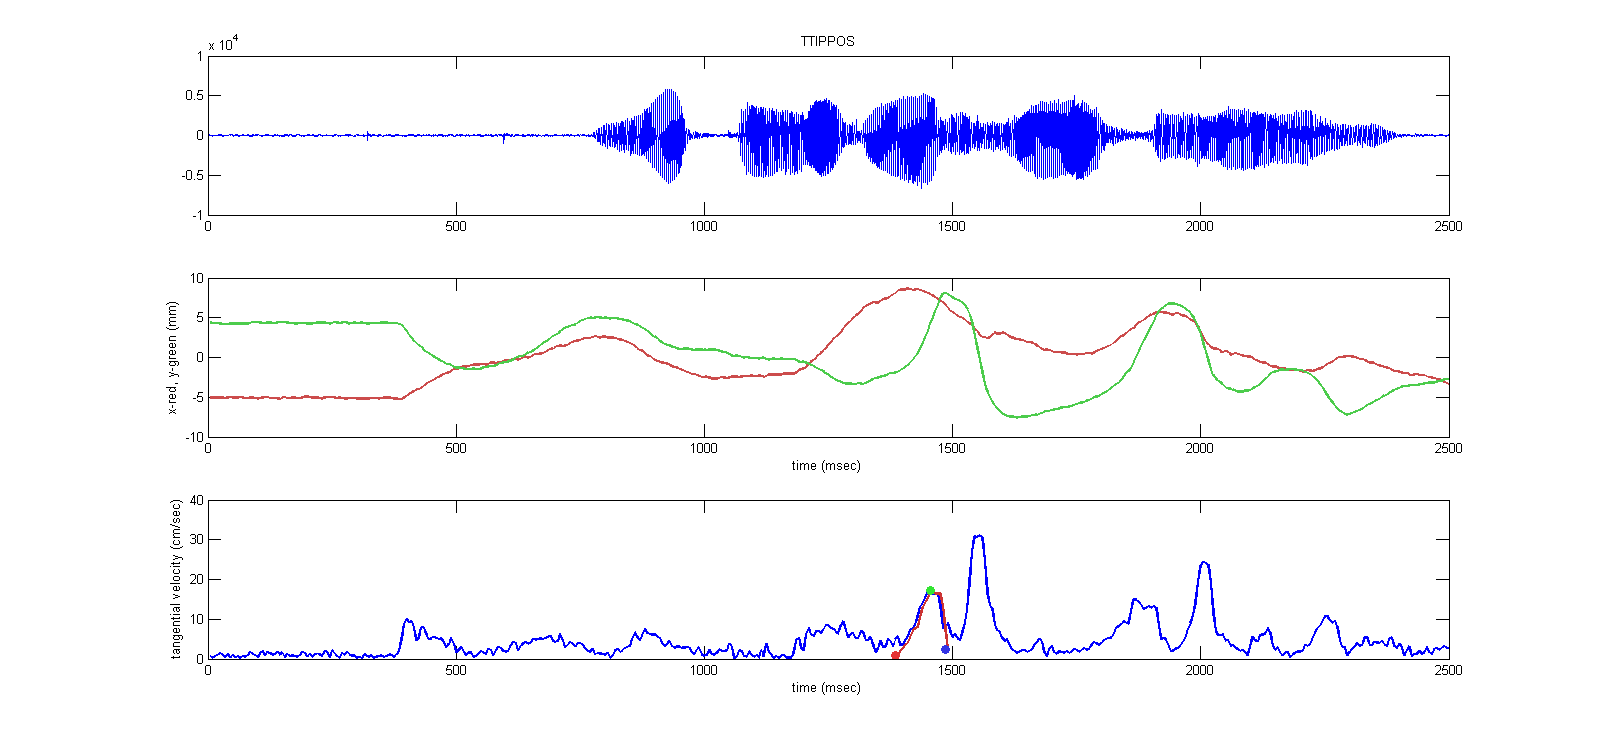
\includegraphics[width=.8\textwidth]{p3.png}
\caption{The velocity profile along the principal component \texttt{u} of movement is plotted red in the GUI over the interval from the left edge \texttt{le} to the right edge \texttt{re} of the movement. This is the peak velocity of interest. The peak velocity is plotted as a green dot, and the left and right edges are marked by a red and a blue dot, respectively.}
\label{fig:velocityprofile}
\end{figure}
We can now calculate summary information about the velocity profile. We find, for instance, its temporal duration \texttt{dur} as follows.
\begin{verbatim}
dur = re - le;
\end{verbatim}
The value we obtain for \texttt{dur} is \texttt{100} milliseconds. The amplitude \texttt{amp} of movement is found as follows.
\begin{verbatim}
x_le = x(ms2sampl(le,srate),1); x_re = x(ms2sampl(re,srate),1);
y_le = x(ms2sampl(le,srate),2); y_re = x(ms2sampl(re,srate),2);
amp = sqrt((x_le - x_re).^2 + (y_le - y_re).^2);
\end{verbatim}
and the amplitude \texttt{proj\_amp} of \texttt{x} projected onto its principal component \texttt{u} is found as follows.
\begin{verbatim}
if ~isempty(u)
    proj_u_x = (u * x.').';
    proj_u_x_le = proj_u_x(ms2sampl(le,srate)); 
    proj_u_x_re = proj_u_x(ms2sampl(re,srate));
    proj_amp = abs(proj_u_x_le - proj_u_x_re);
else
    proj_amp = [];
end
\end{verbatim}
The amplitude \texttt{amp} is \texttt{10.1447} millimeters and the amplitude \texttt{proj\_amp} along the principal component \texttt{u} is \texttt{10.0536} millimeters. This concludes our discussion of this landmark finding algorithm.

\subsection{Scaling up the landmark finder}
\label{subsec:mtSet}

Section~\ref{subsec:oneMT} described an algorithm for delimiting an interval on a single movement trace using kinematic quantities measured on that movement trace. This section applies this algorithm to a set of movement traces and writes a .txt file with the quantites measured over these intervals.\footnote{The MATLAB demo file is AnalyzeTypeDemo.m in the directory util.} First, set a file name. 
\begin{verbatim}
dataFileName = 'demoOutput.txt' ;
\end{verbatim}
The file will be written out to the current directory. The MATLAB constant \texttt{cd} is a string variable whose value is that of the current directory. 
\begin{verbatim}
fileOutputDir = cd;
fileInputDir = cd;
\end{verbatim}
% The asterisk * indicates the wildcard in regular expressions. It stands
% in for other character(s).
% We analyze three bulha tokens.
Now assign to \texttt{srchStr} the substring which is common to all the .mat files containing the movement traces we will analyze.
\begin{verbatim}
srchStr = 'data/*_bulha_*';
\end{verbatim}
The output files will indicate the type of movement trace and the subject who produced it. Assign these names to the variables \texttt{type} and \texttt{subj}, respectively.
\begin{verbatim}
type = 'bulha';
subj = 'mySubj';
\end{verbatim}
The articulator which we are analyzing is the tongue back. The files which we analyze indicate this as \texttt{t\_back\_pos}. Assign this string to the variable \texttt{articulator}.
\begin{verbatim}
articulator = 't_back_pos';
\end{verbatim}
As in Section~\ref{subsec:oneMT}, the analysis of the movement traces depends on a parameter set. Assign these to the variable \texttt{options}.
\begin{verbatim}
options = {[],10,.8,'threshold','pcaProj',80};
\end{verbatim}
Select the landmark you want to analyze in the three bulha tokens. Click on the point you want to analyze in the bottom panel of the GUI, as in Section~\ref{subsec:oneMT}. For this demo, we recommend you choose the large velocity peak, which corresponds to the tongue body movement for the \textipa{/a/} constriction.
\begin{verbatim}
analyzeType(dataFileName, srchStr, type, subj, fileOutputDir, ...
    fileInputDir, articulator, options);
\end{verbatim}
This concludes our application of the landmark finding algorithm to a set of movement traces.

Now look in your current directory for the .txt files with the string demoOutput in the name. There are three files, one which contains measured kinematic quantities, a second which contains velocity profiles, and a third which contains time-normalized velocity profiles. These files can now be taken to a statistical analysis.
 
\clearpage
\thispagestyle{empty}
\bibliographystyle{apa}
\bibliography{matlab}
\nocite{*}
\addcontentsline{toc}{section}{References}



\end{document}